We illustrate with simulations the phase transition phenomena in the chi-square model, and compare numerically the required signal sizes in support recovery problems between the two types of alternatives in the additive error model.  
% These results can provide further guidance to practitioners on when to expect genetic association discoveries. 
% We also demonstrate the fundamental trade-off between odds ratios and relative frequencies in association studies, as outlined in Proposition \ref{prop:signal-size-odds-ratio} and Corollary \ref{cor:signal-size-odds-ratio-conditional-frequency}, using evidence from large-scale genetic studies.

\subsection{Exact support recovery} \label{sec:ch7-exact-support-numerics}

The sparsity of the signal vectors in the experiments are parametrized as in \eqref{eq:signal-sparsity}. 
Signal sizes are assumed equal with magnitude $\lambda(i)=2r\log{p}$ for $i\in S$.
We estimate the support set $S$ using Bonferroni's procedure with nominal FWER level set at $1/(5{\log{p}})$.
The nominal FWER levels vanishes slowly, in line with the assumptions in Theorem \ref{thm:chi-squared-exact-boundary}.
Experiments were repeated 1000 times at each of the 400 sparsity-signal-size combinations, 
%for dimensions $p=10^2, 10^3$, and $10^4$.
for dimension $p=10^4$.

The empirical probabilities of exact support recovery under Bonferroni's procedure are shown in Figure \ref{fig:phase-simulated-chi-squared}.
The numerical results suggest good accuracy of the predicted boundaries in high-dimensions 
(left panels of Figure \ref{fig:phase-simulated-chi-squared}).
%but also practical relevance of the theoretical predictions in moderate dimensions 
%($p=100$, left panels of Figure \ref{fig:phase-simulated-chi-squared}).

\begin{figure}
	\centering
	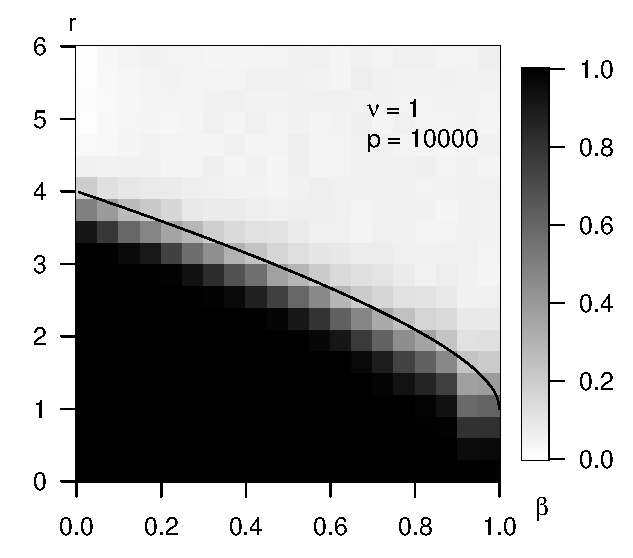
\includegraphics[width=0.32\textwidth]{sim_strong_boundary/simulated_strong_boundary_chi-squared_nu1_p10000.eps}
    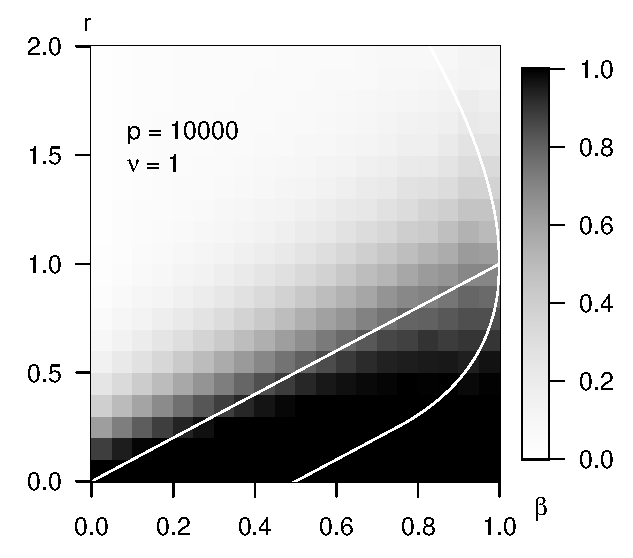
\includegraphics[width=0.32\textwidth]{sim_weak_boundary/simulated_weak_boundary_chi-squared_nu1_p10000.eps}
    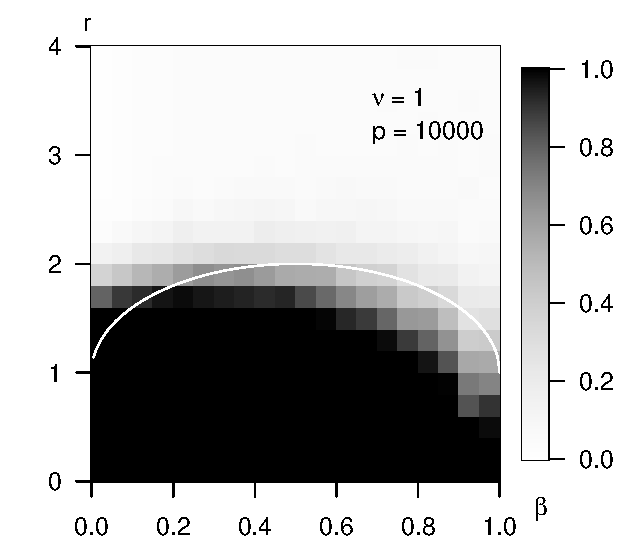
\includegraphics[width=0.32\textwidth]{sim_approx-exact_boundary/simulated_approx-exact_boundary_chi-squared_nu1_p10000.eps}
    
	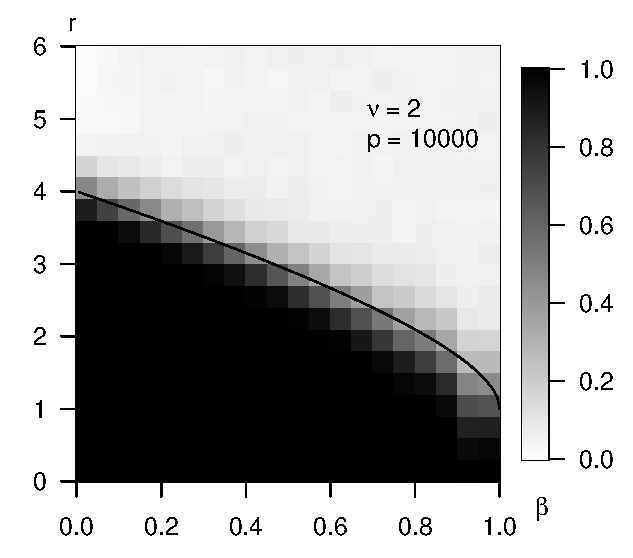
\includegraphics[width=0.32\textwidth]{sim_strong_boundary/simulated_strong_boundary_chi-squared_nu2_p10000.eps}
    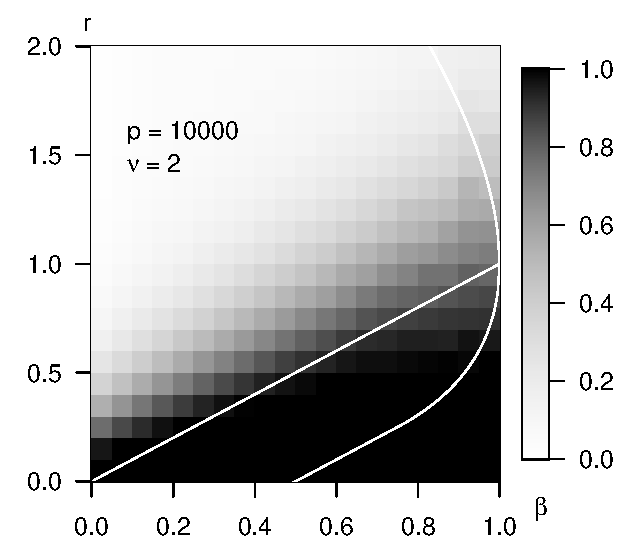
\includegraphics[width=0.32\textwidth]{sim_weak_boundary/simulated_weak_boundary_chi-squared_nu2_p10000.eps}
    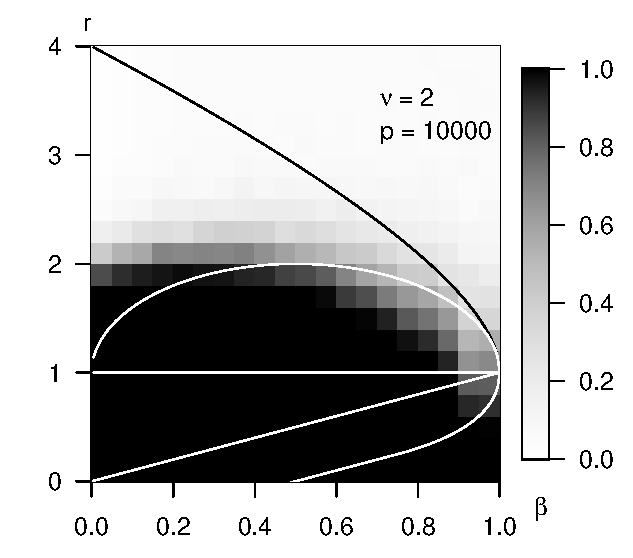
\includegraphics[width=0.32\textwidth]{sim_approx-exact_boundary/simulated_approx-exact_boundary_chi-squared_nu2_p10000.eps}
	
	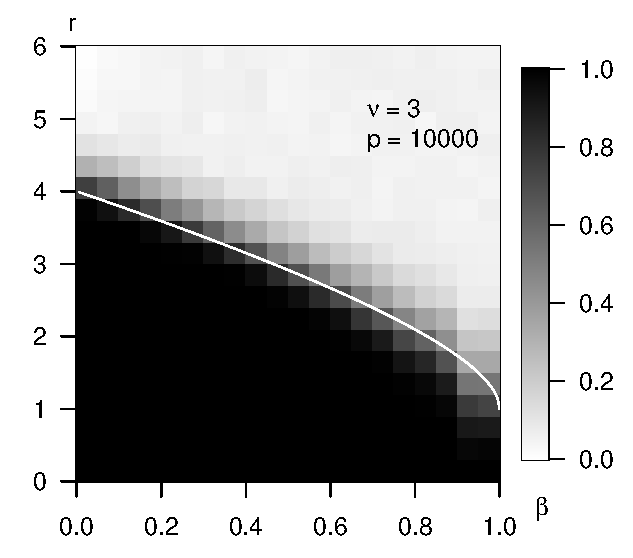
\includegraphics[width=0.32\textwidth]{sim_strong_boundary/simulated_strong_boundary_chi-squared_nu3_p10000.eps}
    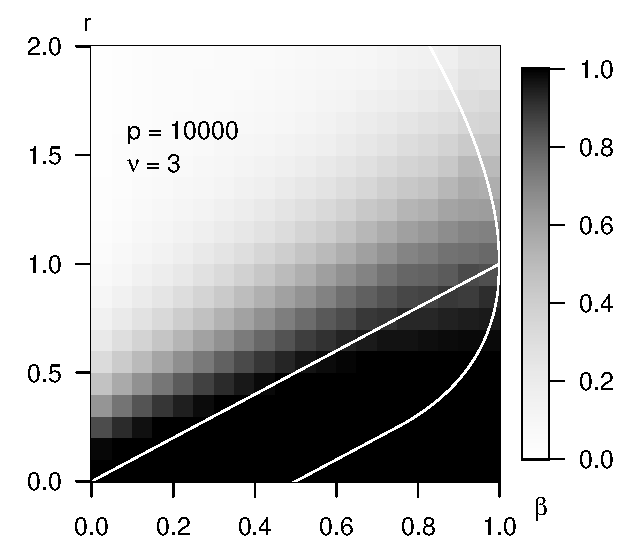
\includegraphics[width=0.32\textwidth]{sim_weak_boundary/simulated_weak_boundary_chi-squared_nu3_p10000.eps}
    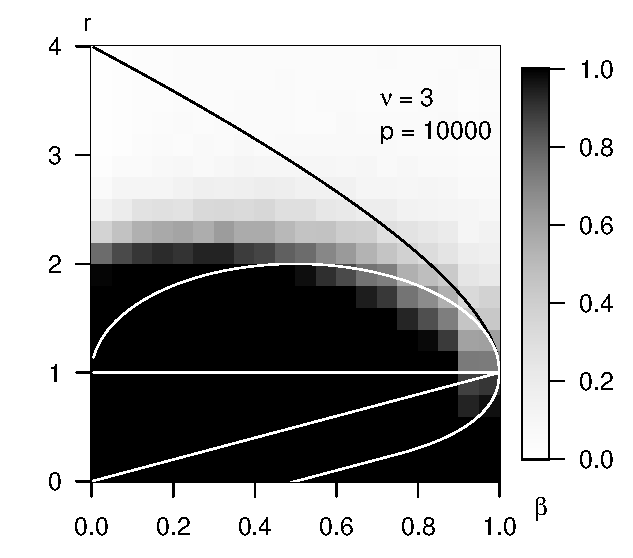
\includegraphics[width=0.32\textwidth]{sim_approx-exact_boundary/simulated_approx-exact_boundary_chi-squared_nu3_p10000.eps}
	
	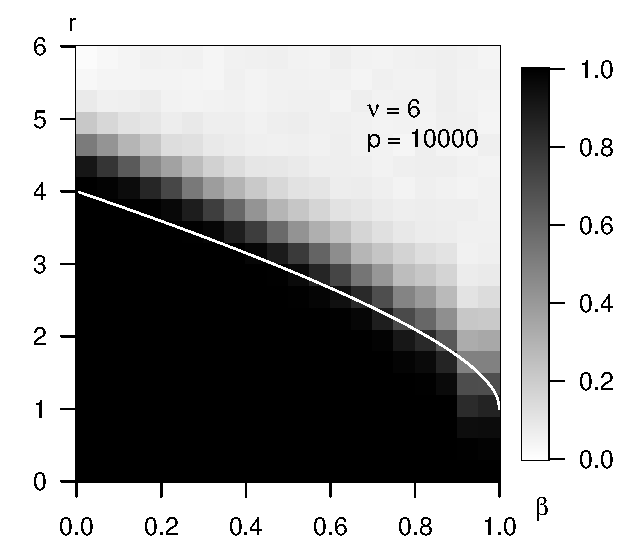
\includegraphics[width=0.32\textwidth]{sim_strong_boundary/simulated_strong_boundary_chi-squared_nu6_p10000.eps}
    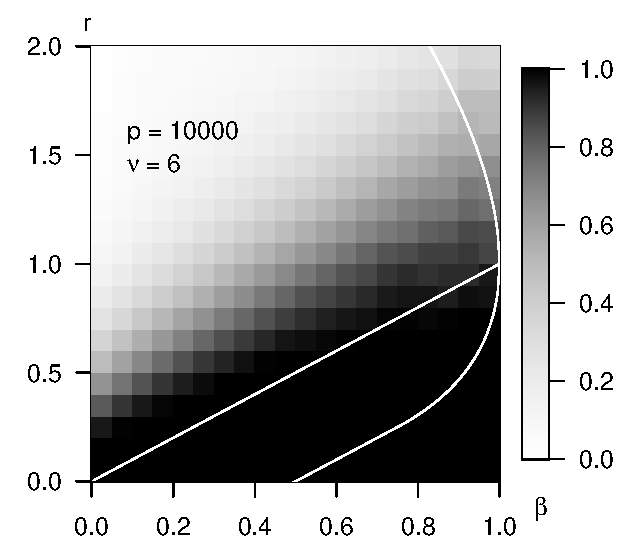
\includegraphics[width=0.32\textwidth]{sim_weak_boundary/simulated_weak_boundary_chi-squared_nu6_p10000.eps}
    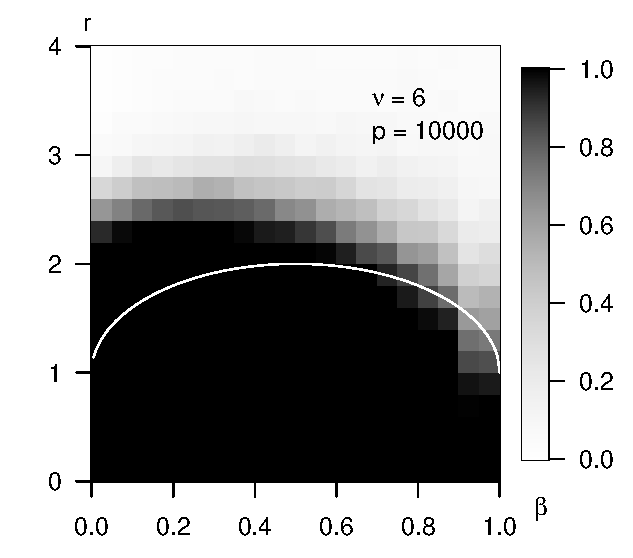
\includegraphics[width=0.32\textwidth]{sim_approx-exact_boundary/simulated_approx-exact_boundary_chi-squared_nu6_p10000.eps}
	\caption{The empirical risks of exact, approximate, and approximate-exact support recovery (left to right) in the chi-squared model \eqref{eq:model-chisq} with Bonferroni's procedure and the Benjamini-Hochberg procedure. 
		We display results as a heatmap for $\nu=1, 2, 3, 6$ (first to last row) at dimension $p=10^4$ (left to right column), for a grid of sparsity levels $\beta$ and signal sizes $r$.
		The experiments were repeated 1000 times for each sparsity-signal size combination; darker color indicates higher probability of exact support recovery.  
		Numerical results are in general agreement with the boundaries described in Theorem \ref{thm:chi-squared-exact-boundary}; for large $\nu$'s, the phase transitions take place somewhat above the predicted boundaries.} 
	\label{fig:phase-simulated-chi-squared}
\end{figure}



%\begin{figure}
%      \centering
%      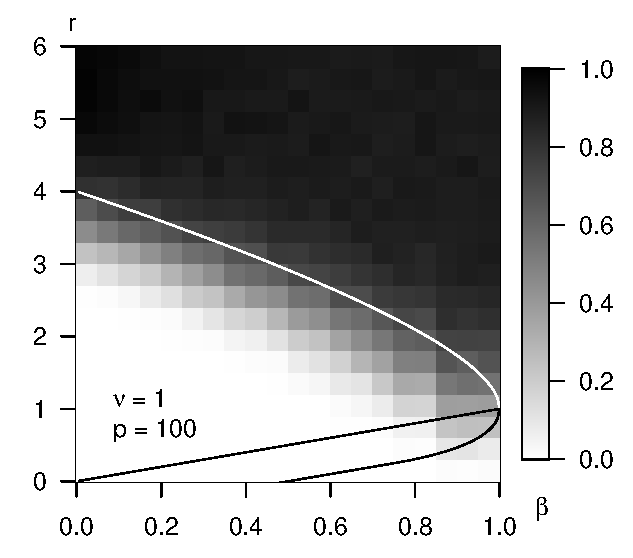
\includegraphics[width=0.32\textwidth]{sim_strong_boundary/simulated_phase_diagram_chi-squared_nu1_p100.eps}
%      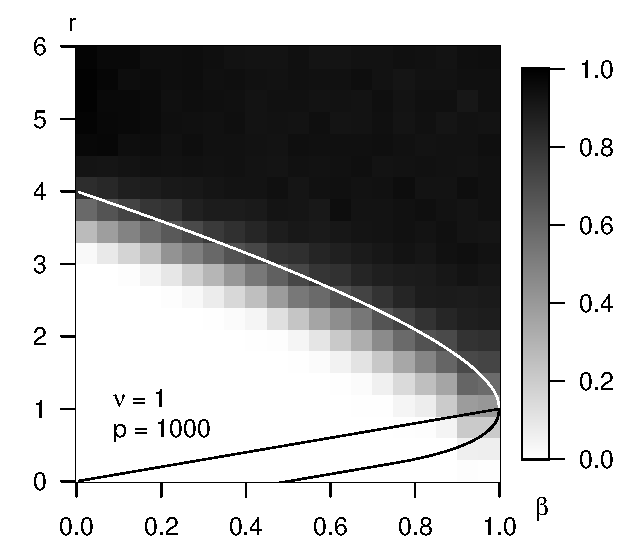
\includegraphics[width=0.32\textwidth]{sim_strong_boundary/simulated_phase_diagram_chi-squared_nu1_p1000.eps}
%      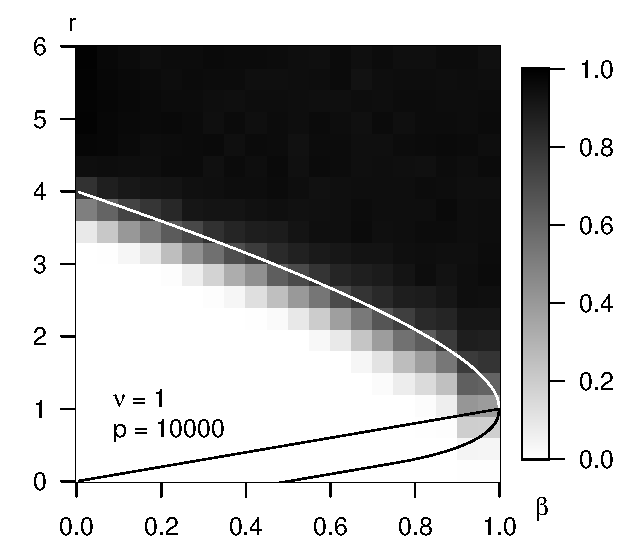
\includegraphics[width=0.32\textwidth]{sim_strong_boundary/simulated_phase_diagram_chi-squared_nu1_p10000.eps}
%      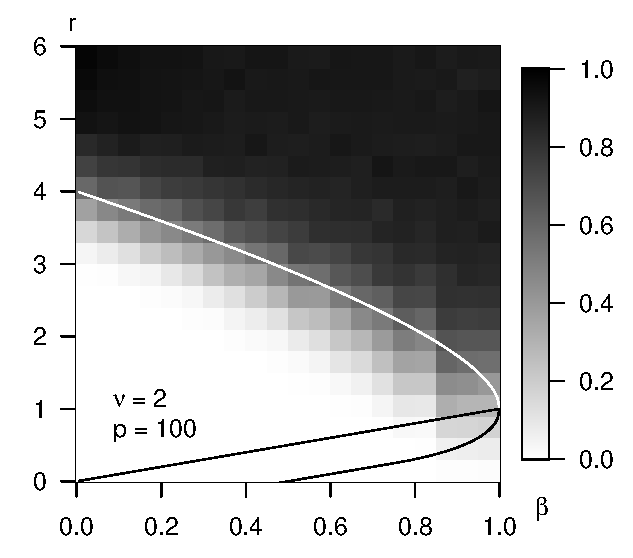
\includegraphics[width=0.32\textwidth]{sim_strong_boundary/simulated_phase_diagram_chi-squared_nu2_p100.eps}
%      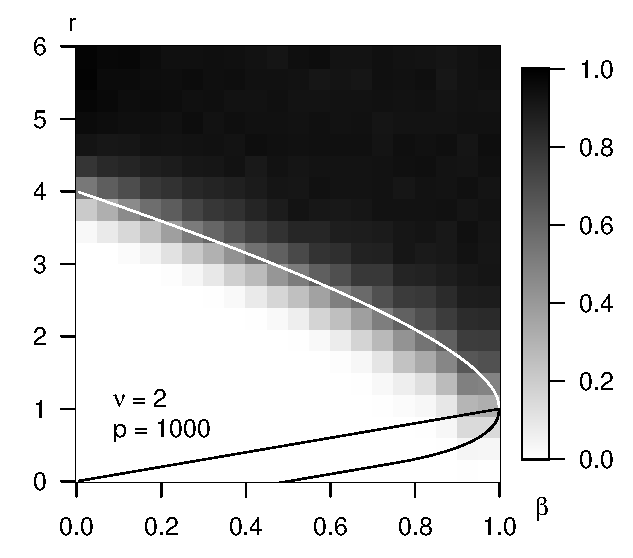
\includegraphics[width=0.32\textwidth]{sim_strong_boundary/simulated_phase_diagram_chi-squared_nu2_p1000.eps}
%      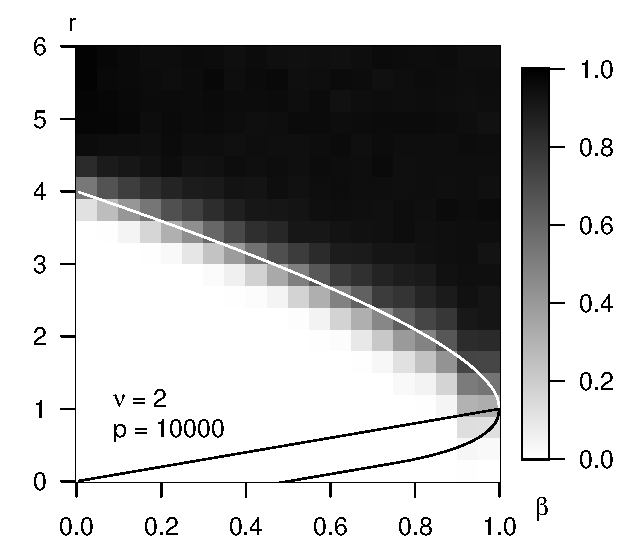
\includegraphics[width=0.32\textwidth]{sim_strong_boundary/simulated_phase_diagram_chi-squared_nu2_p10000.eps}
%      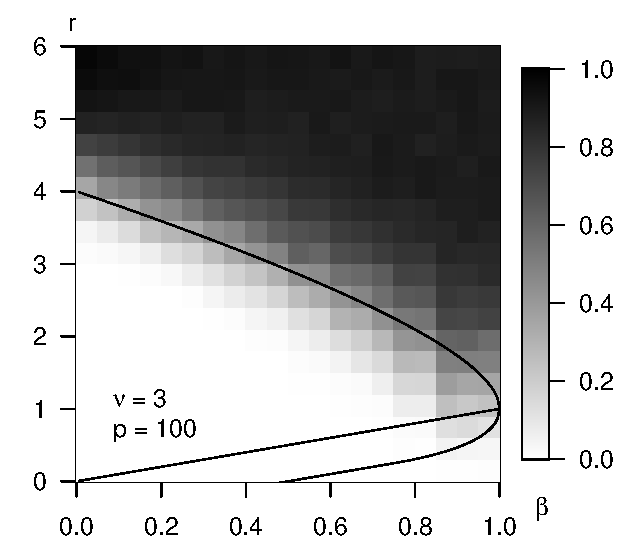
\includegraphics[width=0.32\textwidth]{sim_strong_boundary/simulated_phase_diagram_chi-squared_nu3_p100.eps}
%      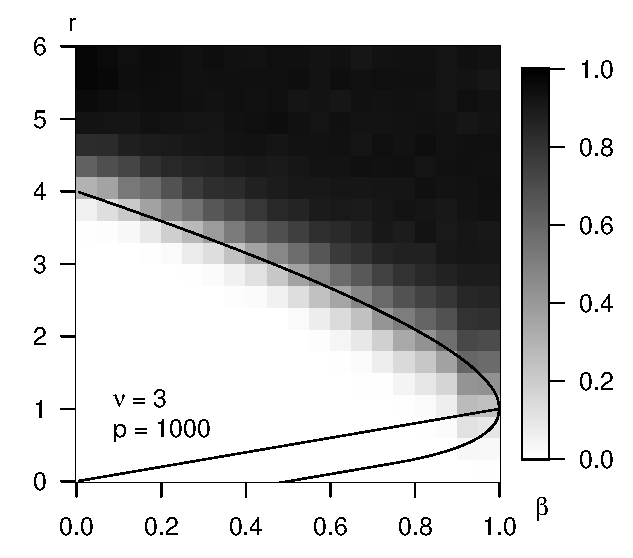
\includegraphics[width=0.32\textwidth]{sim_strong_boundary/simulated_phase_diagram_chi-squared_nu3_p1000.eps}
%      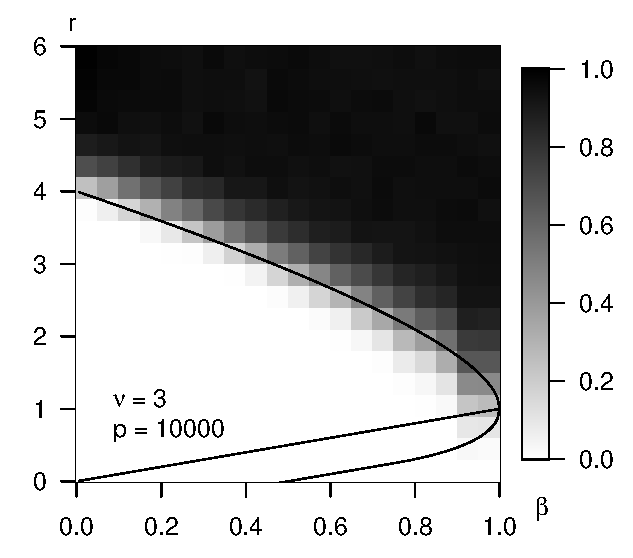
\includegraphics[width=0.32\textwidth]{sim_strong_boundary/simulated_phase_diagram_chi-squared_nu3_p10000.eps}
%      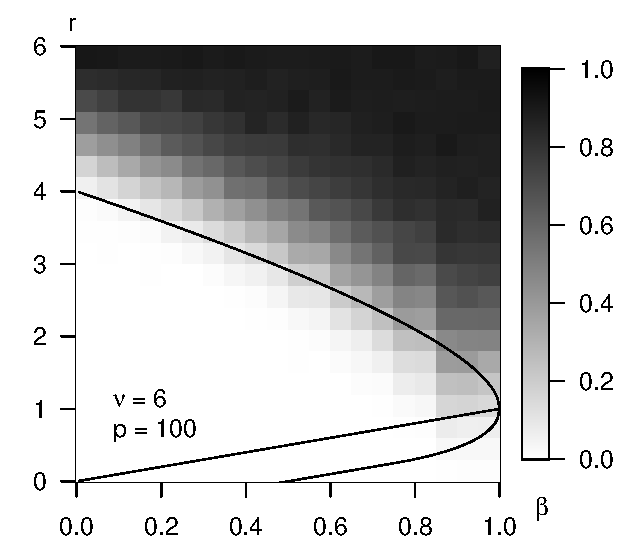
\includegraphics[width=0.32\textwidth]{sim_strong_boundary/simulated_phase_diagram_chi-squared_nu6_p100.eps}
%      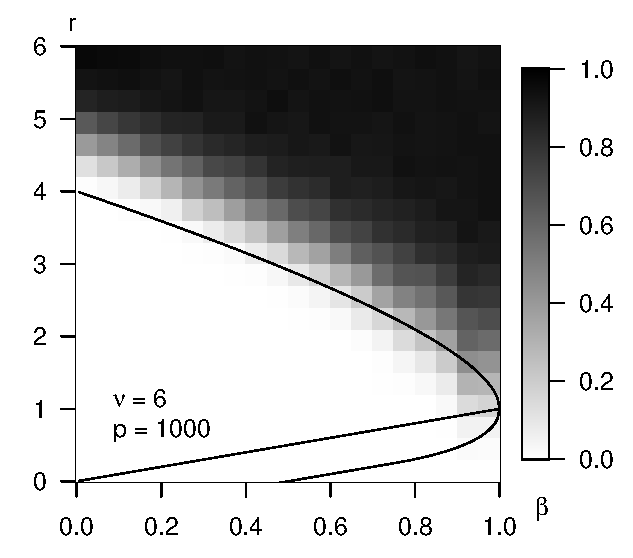
\includegraphics[width=0.32\textwidth]{sim_strong_boundary/simulated_phase_diagram_chi-squared_nu6_p1000.eps}
%      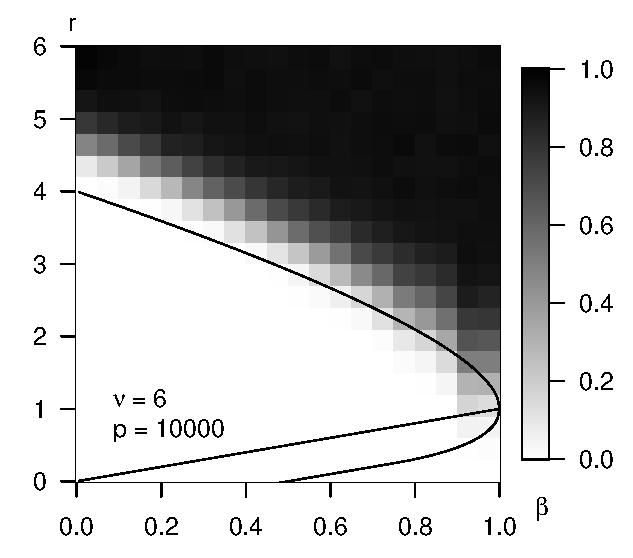
\includegraphics[width=0.32\textwidth]{sim_strong_boundary/simulated_phase_diagram_chi-squared_nu6_p10000.eps}
%      \caption{The empirical probability of exact support recovery of Bonferroni's procedure in the chi-squared model \eqref{eq:model-chisq}. 
%      We simulate $\nu=1, 2, 3, 6$ (first to last row), at dimensions $p=10^2, 10^3, 10^4$ (left to right column), for a grid of sparsity levels $\beta$ and signal sizes $r$.
%      The experiments were repeated 1000 times for each sparsity-signal size combination; darker color indicates higher probability of exact support recovery.  
%      Numerical results are in general agreement with the boundaries described in Theorem \ref{thm:chi-squared-exact-boundary}; for large $\nu$'s, the phase transitions take place somewhat above the predicted boundaries.
%      The boundary for the approximate support recovery (Theorem \ref{thm:chi-squared-approx-boundary}) and the detection boundary (see Donoho and Jin (2004)) are plotted for comparison.} 
%      \label{fig:phase-simulated-chi-squared}
%\end{figure}

We conduct further experiments to examine the optimality claims in Theorem \ref{thm:chi-squared-exact-boundary} by comparing with the oracle procedure with thresholds $t_p=\min_{i\in S}x(i)$.
We also examine the claims in Section \ref{subsec:one-vs-two-sided}, and compare the one-sided alternatives in Gaussian additive models with the two-sided alternatives (or equivalently, the chi-square model with $\nu=1$).
We apply Bonferroni's procedure and the oracle thresholding procedure in both settings.

The experiments were repeated 1000 times for a grid of signal size values ranging from $r=0$ to $6$, and for dimensions $10^2, 10^3$, and $10^5$.
Results of the experiments, shown in Figure \ref{fig:one-vs-two-sided-exact_support_recovery}, suggest vanishing difference between difficulties of two-sided vs one-sided alternatives in the additive error models, as well as vanishing difference between the powers of Bonferroni's procedures and the oracle procedures as $p\to\infty$.

\begin{figure}
      \centering
      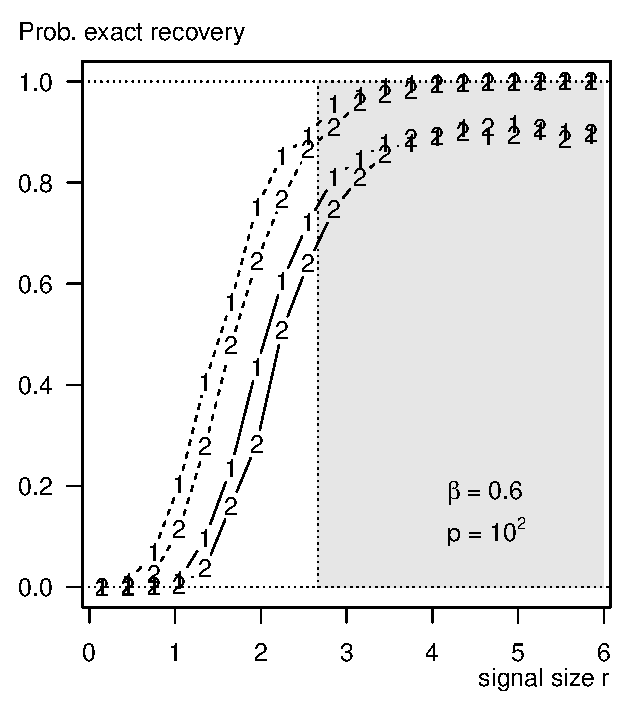
\includegraphics[width=0.32\textwidth]{sim_one-vs-two-sided/exact_recovery_one-vs-two-sided_beta06_p100.eps}
      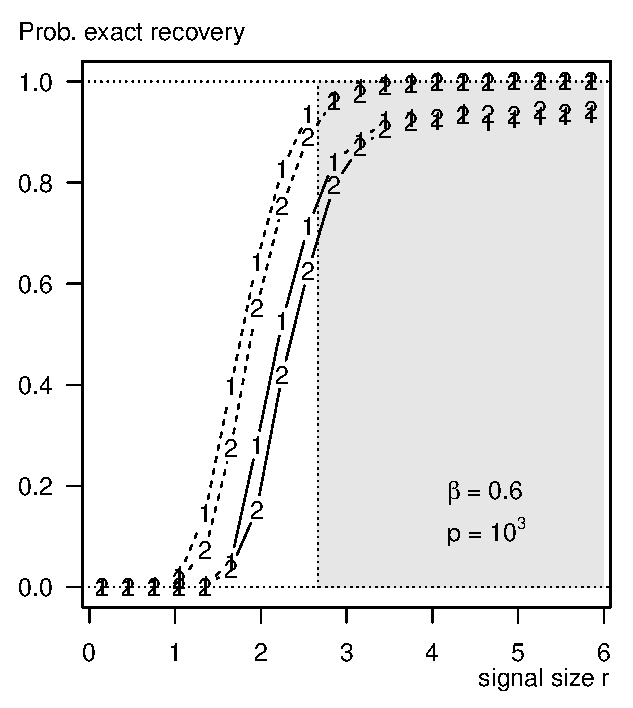
\includegraphics[width=0.32\textwidth]{sim_one-vs-two-sided/exact_recovery_one-vs-two-sided_beta06_p1000.eps}
      % 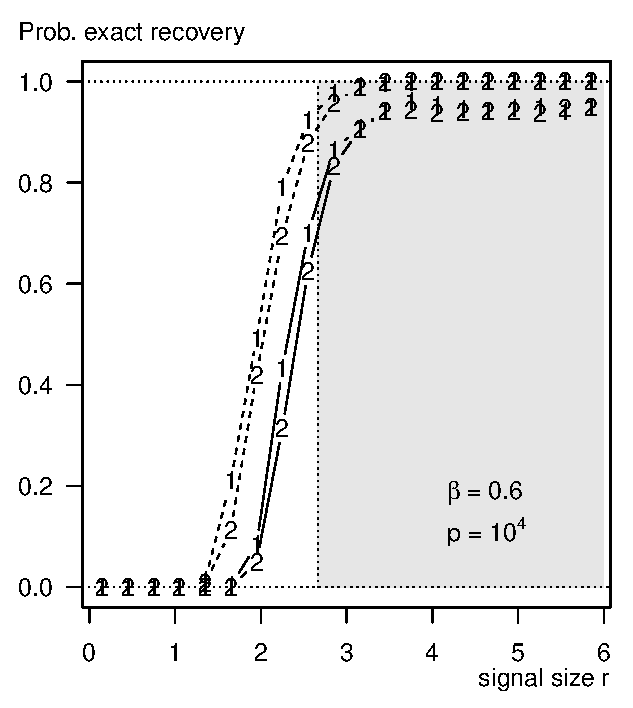
\includegraphics[width=0.33\textwidth]{sim_one-vs-two-sided/exact_recovery_one-vs-two-sided_beta06_p10000.eps}
      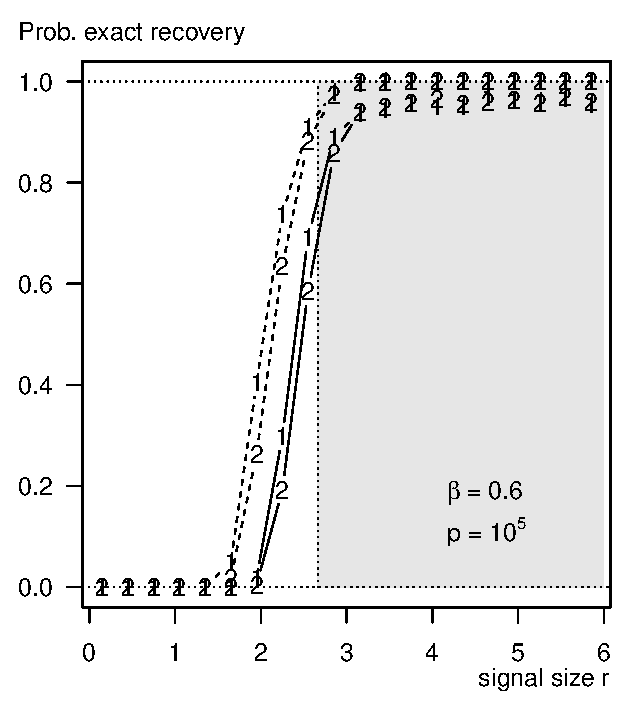
\includegraphics[width=0.32\textwidth]{sim_one-vs-two-sided/exact_recovery_one-vs-two-sided_beta06_p100000.eps}
      \caption{The empirical probability of exact support recovery of Bonferroni's procedure (solid curves) and the oracle procedure (dashed curves) in the chi-squared model with one degree of freedom (marked `2') in the additive Gaussian error model and under one-sided alternatives (marked `1'). 
      We simulate at dimensions $p=10^2, 10^3, 10^5$ (left to right) for a grid of signal sizes $r$ and sparsity level $\beta=0.6$.
      The experiments were repeated 1000 times for each method-model-signal-size combination. 
      Numerical results show evidence of convergence to the 0-1 law as predicted by Theorem \ref{thm:chi-squared-exact-boundary}; regions where asymptotically exact support recovery can be achieved are shaded in grey.
      The difference in power between Bonferroni's procedure and the oracle procedure, as well as in the two types of alternatives both decrease as dimensionality increases.} 
      \label{fig:one-vs-two-sided-exact_support_recovery}
\end{figure}

\subsection{Approximate, and approximate-exact support recovery}

Similar experiments are conducted to examine the optimality claims in Theorem \ref{thm:chi-squared-approx-boundary}, and in Section \ref{subsec:one-vs-two-sided}.
We define an oracle thresholding procedure for approximate support recovery, where the threshold is chosen to minimize the empirical risk.
That is,
$$
t_p(x, S) \in \argmin_{t\in\R} \frac{|\widehat{S}(t)\setminus S|}{\max\{|\widehat{S}(t)|,1\}} + \frac{|S\setminus \widehat{S}(t)|}{\max\{|{S}|,1\}},
%\mathcal{R^\mathrm{oracle}} \in \argmin_{\widehat{S}(\mathcal{R})\in\mathcal{S}} \mathrm{risk}^{\mathrm{A}}(\mathcal{R}),
$$
where $\widehat{S}(t) = \{i\;|\;x(i)\ge t\}$;
in implementation, we only need to scan the values of observations $t\in\{x(1), \ldots, x(p)\}$. 
The nominal FDR level for the BH procedure is set at $1/(5{\log{p}})$, therefore slowly vanishing, in line with the assumptions in Theorem \ref{thm:chi-squared-approx-boundary}; all other parameters are identical to that in the experiments for exact support recovery in 
Section \ref{sec:ch7-exact-support-numerics}.  The results of the experiments are shown in 
Figure \ref{fig:one-vs-two-sided-approx_support_recovery} and in the middle column of Figure \ref{fig:phase-simulated-chi-squared}.

We also examine the boundary described in Theorem \ref{thm:chi-squared-exact-approx-boundary}.
Experimental settings are identical to that in the experiments for approximate support recovery.
% Results for the BH procedure are in general close to that of the oracle procedure,
We compare the performance of the BH procedure with an oracle procedure with threshold
$$
t_p(x, S) \in \min_{i\in S} x(i),
$$
and visualize the results of the experiments in the right column of Figure \ref{fig:phase-simulated-chi-squared}.
Notice that the BH procedure sets its threshold somewhat higher than the oracle, especially for small $\beta$'s. 
The empirical risk of the oracle procedure (not shown here in the interest of space) follows much more closely the predicted boundary \eqref{eq:approx-exact-boundary-chisquared}.

\begin{figure}
      \centering
      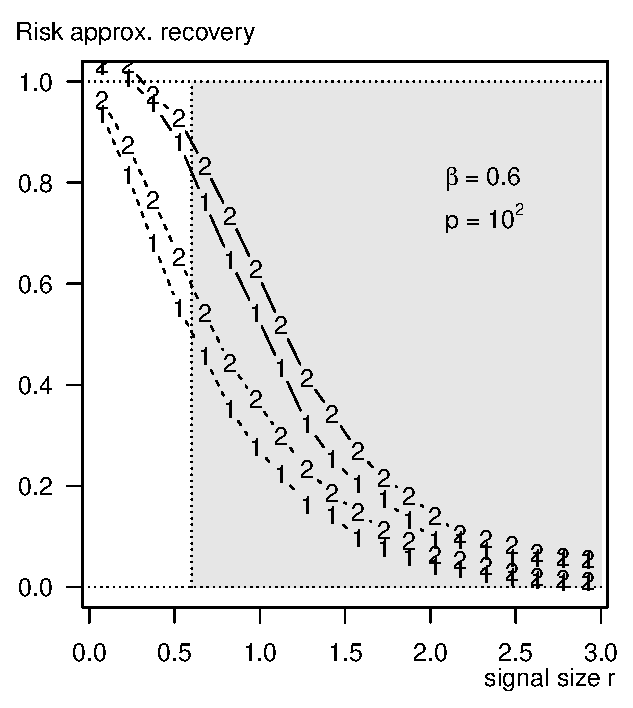
\includegraphics[width=0.32\textwidth]{sim_one-vs-two-sided/approx_recovery_one-vs-two-sided_beta06_p100.eps}
      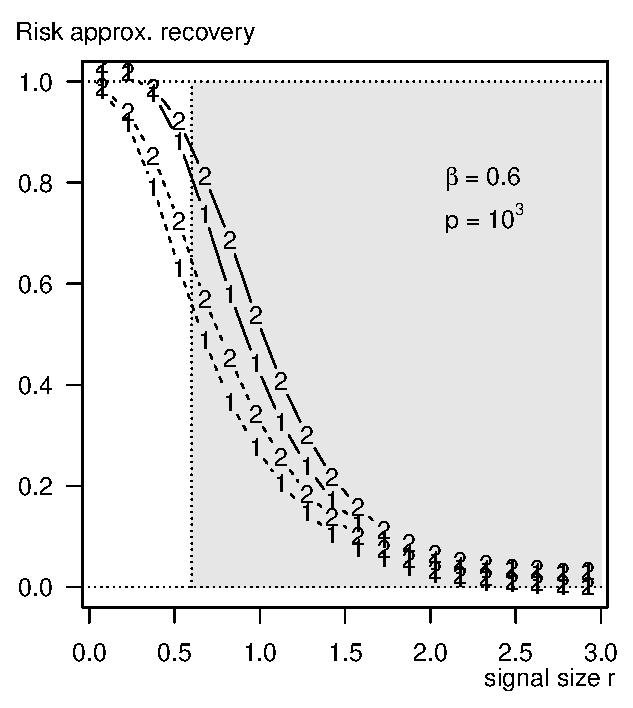
\includegraphics[width=0.32\textwidth]{sim_one-vs-two-sided/approx_recovery_one-vs-two-sided_beta06_p1000.eps}
      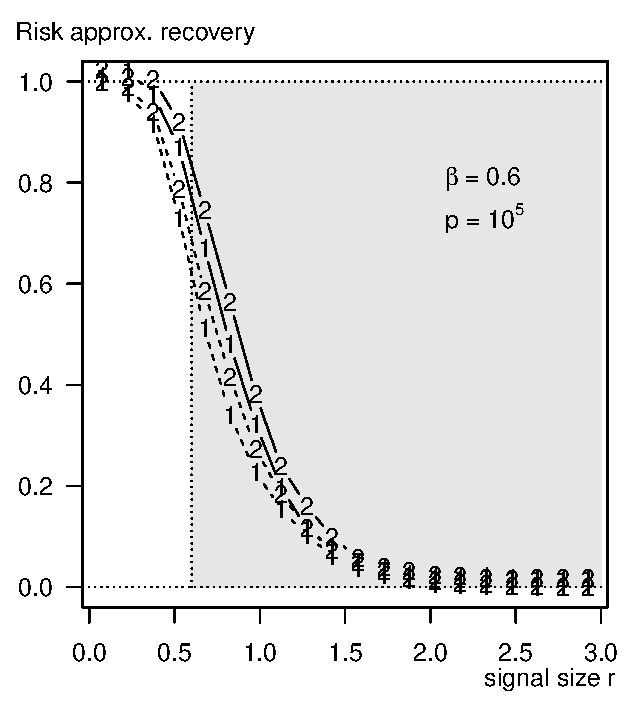
\includegraphics[width=0.32\textwidth]{sim_one-vs-two-sided/approx_recovery_one-vs-two-sided_beta06_p100000.eps}
      \caption{The empirical risk of approximate support recovery of Benjamini-Hochberg's procedure (solid curves) and the oracle procedure (dashed curves) in the chi-squared model with one degree of freedom (marked `2') and in the additive Gaussian error model under one-sided alternatives (marked `1'). 
      We simulate at dimensions $p=10^2, 10^3, 10^5$ (left to right) for a grid of signal sizes $r$ and sparsity level $\beta=0.6$.
      The experiments were repeated 1000 times for each method-model-signal-size combination. 
      Numerical results show evidence of convergence to the 0-1 law as predicted by Theorem \ref{thm:chi-squared-approx-boundary}; regions where asymptotically approximate support recovery can be achieved are shaded in grey.
      The difference in risks between Benjamini-Hochberg's procedure and the oracle procedure, as well as in the two types of alternatives, both decrease as dimensionality increases.} 
      \label{fig:one-vs-two-sided-approx_support_recovery}
\end{figure}

%
%\begin{figure}
%      \centering
%      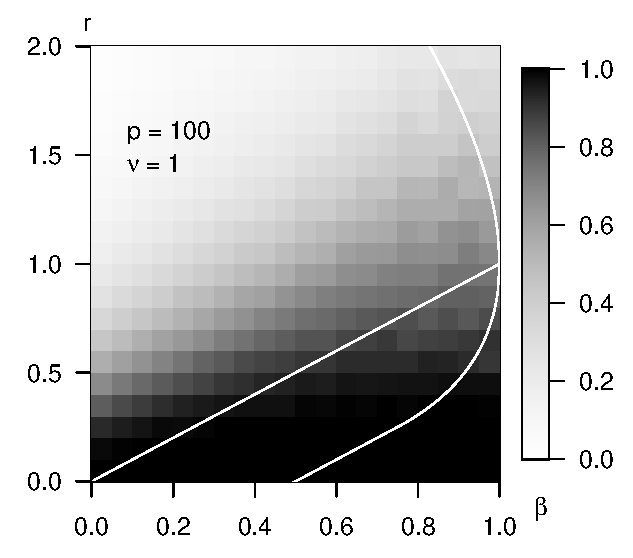
\includegraphics[width=0.32\textwidth]{sim_weak_boundary/simulated_weak_boundary_chi-squared_nu1_p100.eps}
%      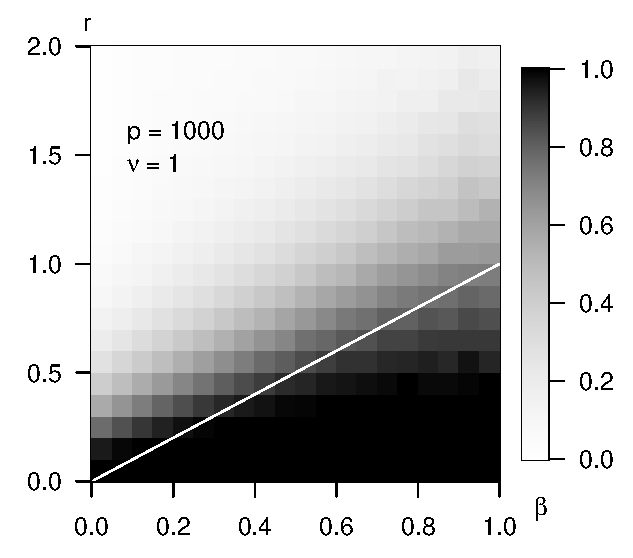
\includegraphics[width=0.32\textwidth]{sim_weak_boundary/simulated_weak_boundary_chi-squared_nu1_p1000.eps}
%      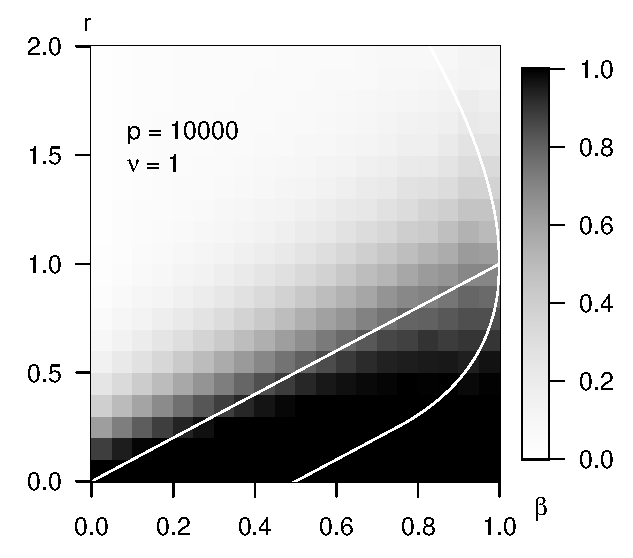
\includegraphics[width=0.32\textwidth]{sim_weak_boundary/simulated_weak_boundary_chi-squared_nu1_p10000.eps}
%      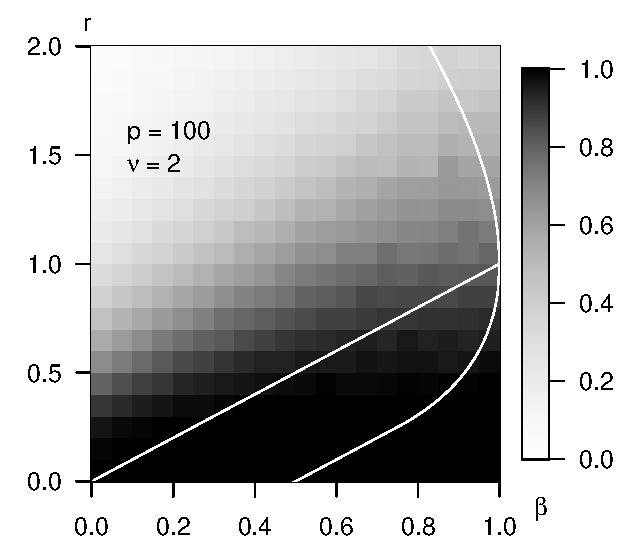
\includegraphics[width=0.32\textwidth]{sim_weak_boundary/simulated_weak_boundary_chi-squared_nu2_p100.eps}
%      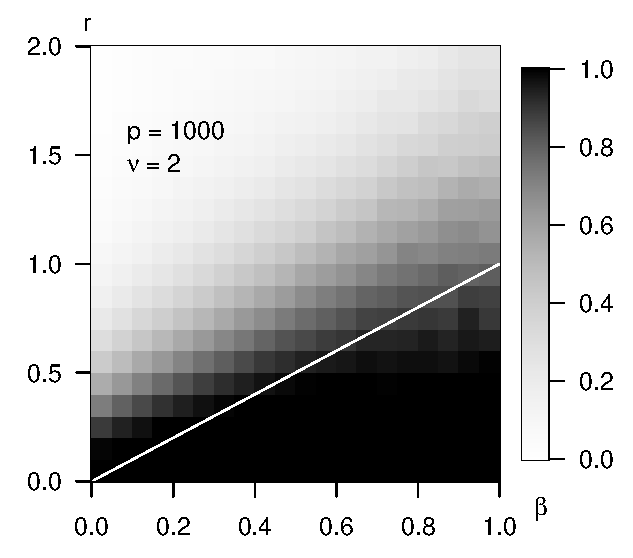
\includegraphics[width=0.32\textwidth]{sim_weak_boundary/simulated_weak_boundary_chi-squared_nu2_p1000.eps}
%      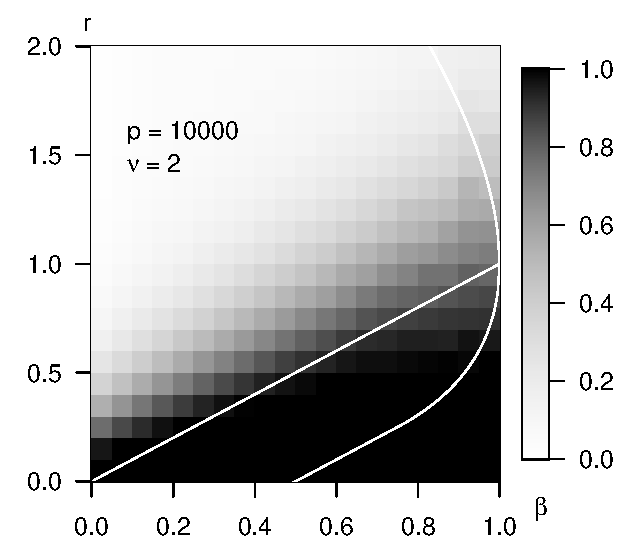
\includegraphics[width=0.32\textwidth]{sim_weak_boundary/simulated_weak_boundary_chi-squared_nu2_p10000.eps}
%      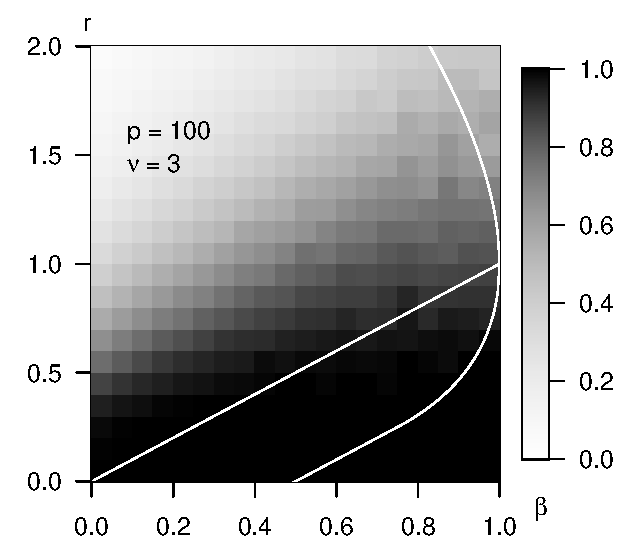
\includegraphics[width=0.32\textwidth]{sim_weak_boundary/simulated_weak_boundary_chi-squared_nu3_p100.eps}
%      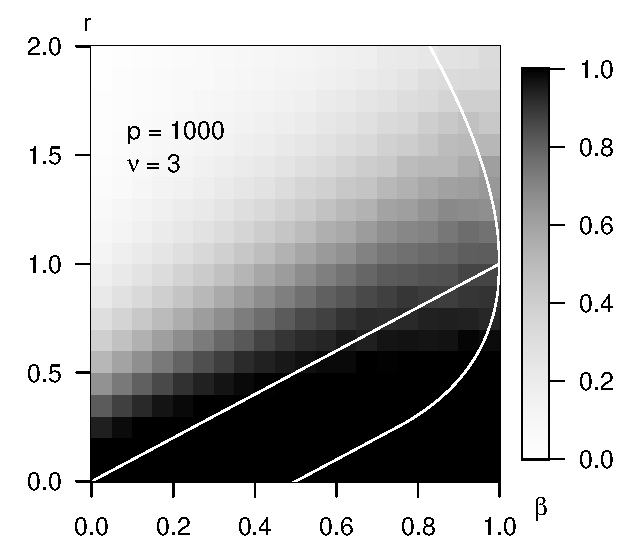
\includegraphics[width=0.32\textwidth]{sim_weak_boundary/simulated_weak_boundary_chi-squared_nu3_p1000.eps}
%      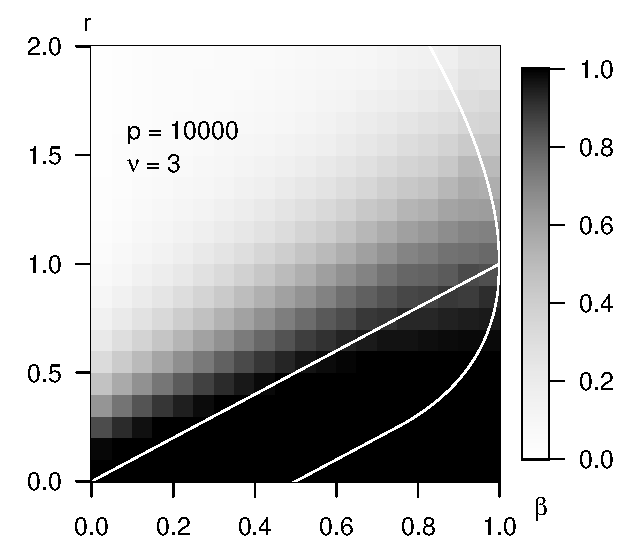
\includegraphics[width=0.32\textwidth]{sim_weak_boundary/simulated_weak_boundary_chi-squared_nu3_p10000.eps}
%      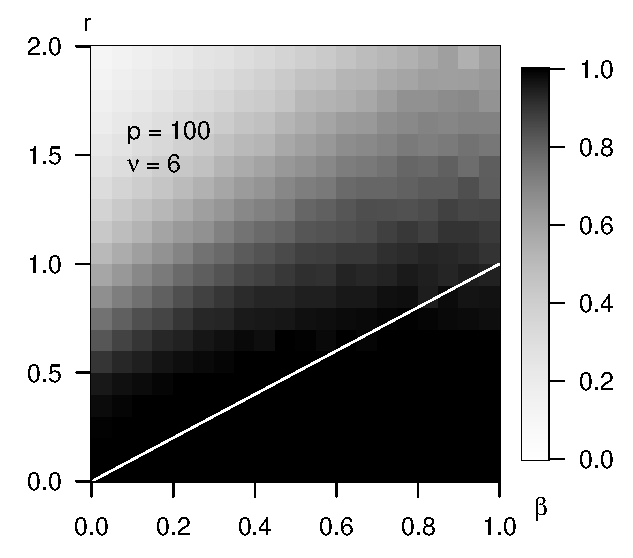
\includegraphics[width=0.32\textwidth]{sim_weak_boundary/simulated_weak_boundary_chi-squared_nu6_p100.eps}
%      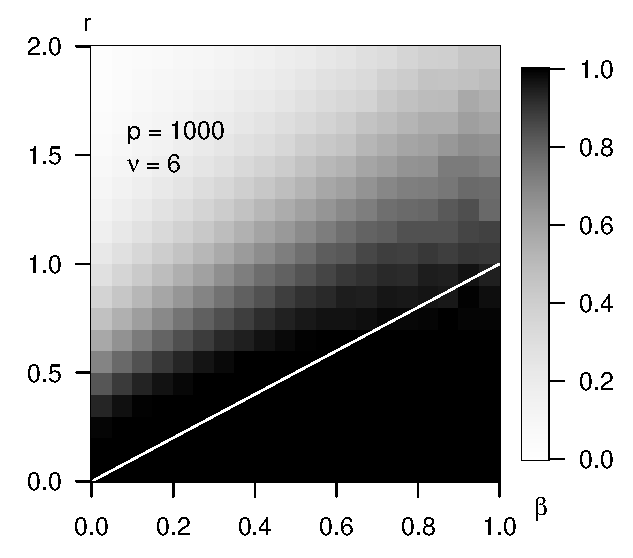
\includegraphics[width=0.32\textwidth]{sim_weak_boundary/simulated_weak_boundary_chi-squared_nu6_p1000.eps}
%      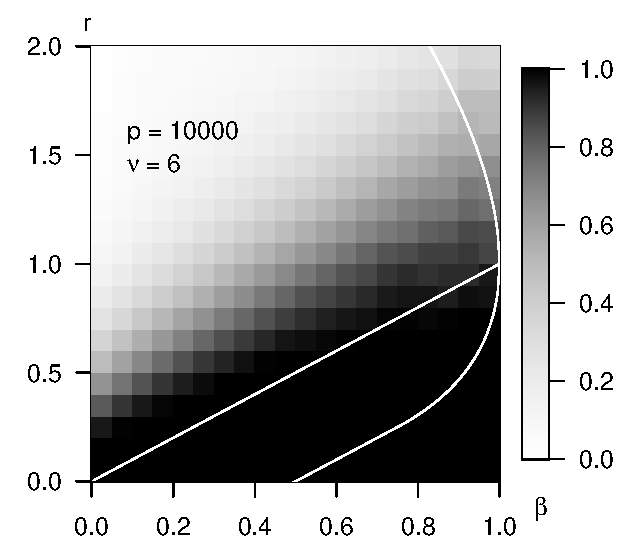
\includegraphics[width=0.32\textwidth]{sim_weak_boundary/simulated_weak_boundary_chi-squared_nu6_p10000.eps}
%      \caption{The estimated risk of approximate support recovery $\mathrm{risk}^{\mathrm{A}}$ (see \eqref{eq:risk-approximate}) of the Benjamini-Hochberg procedure in the chi-squared model \eqref{eq:model-chisq}. 
%      We simulate $\nu=1, 2, 3, 6$ (first to last row), at dimensions $p=10^2, 10^3, 10^4$ (left to right column), for a grid of sparsity levels $\beta$ and signal sizes $r$.
%      The experiments were repeated 1000 times for each sparsity-signal size combination; darker color indicates higher larger $\mathrm{risk}^{\mathrm{A}}$. 
%      Numerical results are generally in agreement with the boundaries described in Theorem \ref{thm:chi-squared-approx-boundary}; for large $\nu$'s, the phase transitions take place somewhat above the predicted boundaries.
%      The boundary for the exact support recovery problem (Theorem \ref{thm:chi-squared-exact-boundary}) and the detection boundary (see Donoho and Jin (2004)) are plotted for comparison.} 
%      \label{fig:phase-simulated-chi-squared-approx-boundary}
%\end{figure}
%
%
%\begin{figure}
%      \centering
%      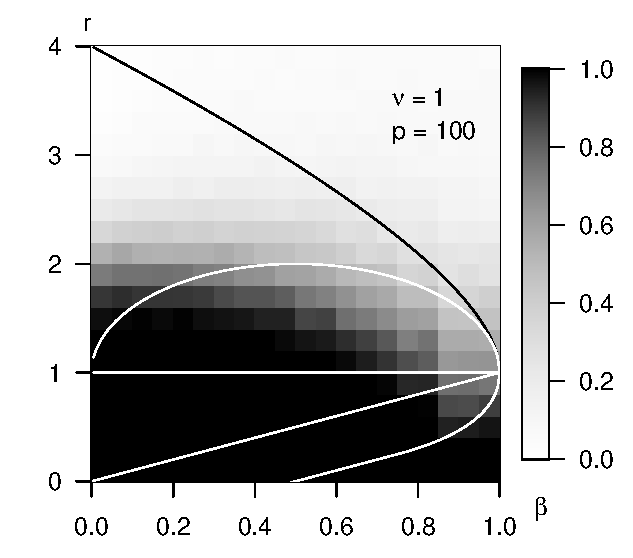
\includegraphics[width=0.32\textwidth]{sim_approx-exact_boundary/simulated_approx-exact_boundary_chi-squared_nu1_p100.eps}
%      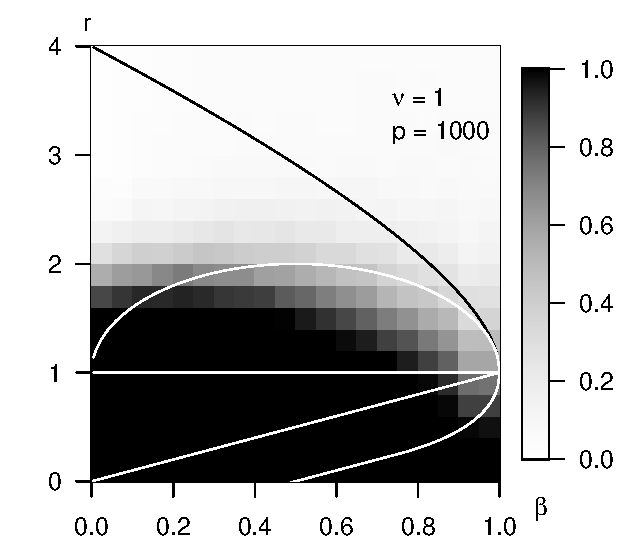
\includegraphics[width=0.32\textwidth]{sim_approx-exact_boundary/simulated_approx-exact_boundary_chi-squared_nu1_p1000.eps}
%      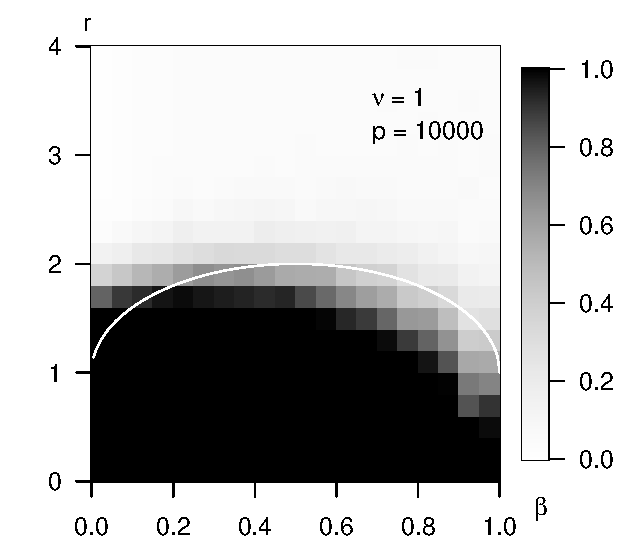
\includegraphics[width=0.32\textwidth]{sim_approx-exact_boundary/simulated_approx-exact_boundary_chi-squared_nu1_p10000.eps}
%      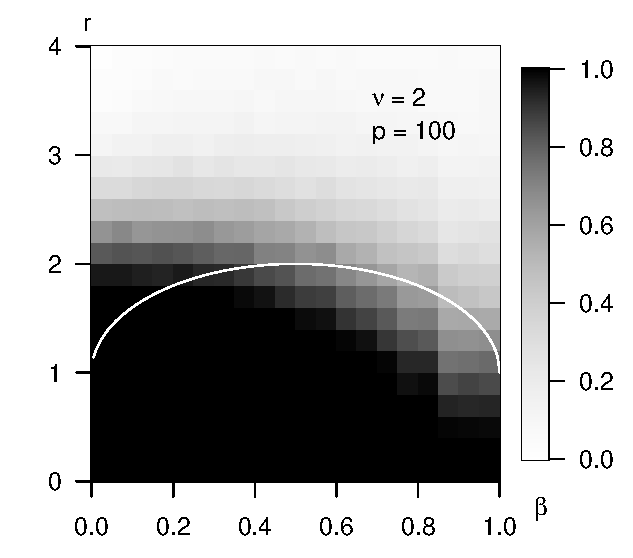
\includegraphics[width=0.32\textwidth]{sim_approx-exact_boundary/simulated_approx-exact_boundary_chi-squared_nu2_p100.eps}
%      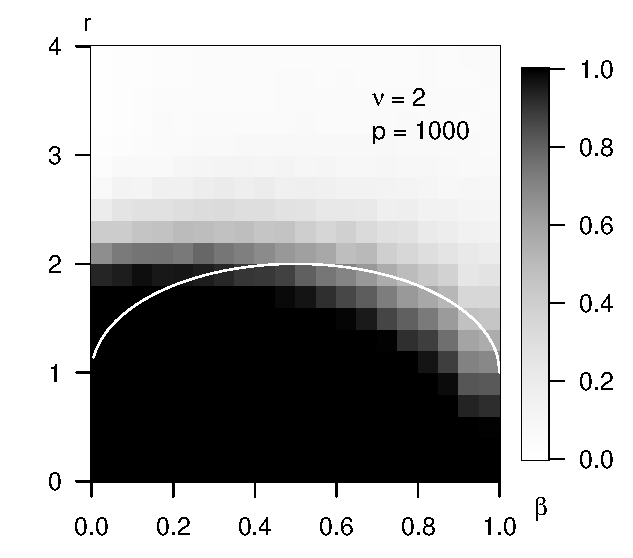
\includegraphics[width=0.32\textwidth]{sim_approx-exact_boundary/simulated_approx-exact_boundary_chi-squared_nu2_p1000.eps}
%      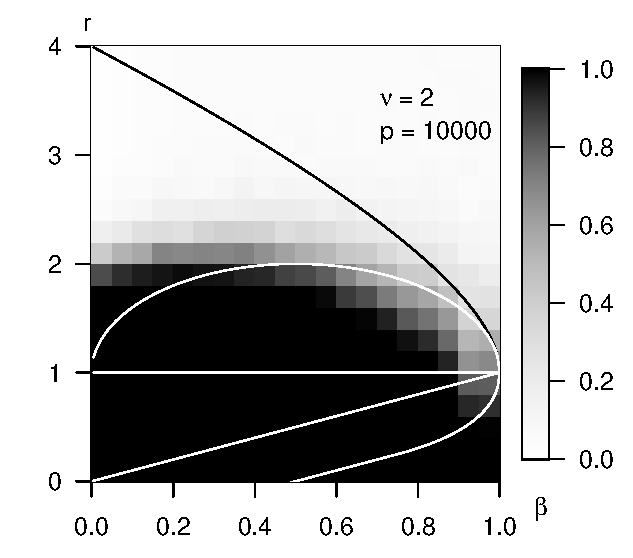
\includegraphics[width=0.32\textwidth]{sim_approx-exact_boundary/simulated_approx-exact_boundary_chi-squared_nu2_p10000.eps}
%      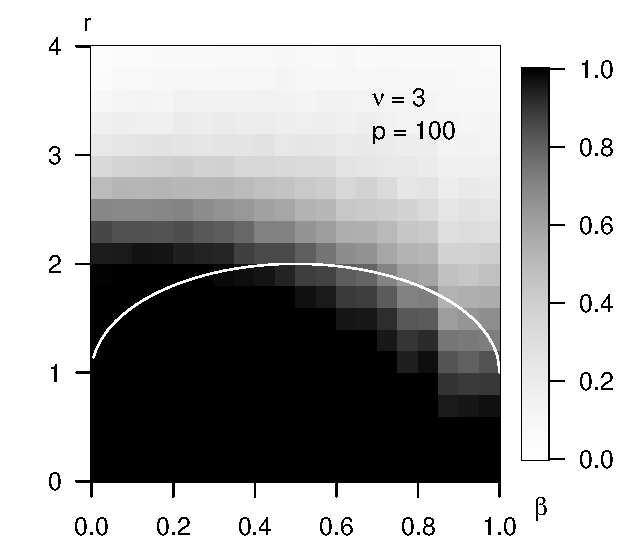
\includegraphics[width=0.32\textwidth]{sim_approx-exact_boundary/simulated_approx-exact_boundary_chi-squared_nu3_p100.eps}
%      \includegraphics[width=0.32\textwidth]{sim_approx-exact_boundary/simulated_approx-exact_boundary_chi-squared_nu3_p1000.eps}
%      \includegraphics[width=0.32\textwidth]{sim_approx-exact_boundary/simulated_approx-exact_boundary_chi-squared_nu3_p10000.eps}
%      \includegraphics[width=0.32\textwidth]{sim_approx-exact_boundary/simulated_approx-exact_boundary_chi-squared_nu6_p100.eps}
%      \includegraphics[width=0.32\textwidth]{sim_approx-exact_boundary/simulated_approx-exact_boundary_chi-squared_nu6_p1000.eps}
%      \includegraphics[width=0.32\textwidth]{sim_approx-exact_boundary/simulated_approx-exact_boundary_chi-squared_nu6_p10000.eps}
%      \caption{The estimated risk of approximate-exact support recovery $\mathrm{risk}^{\mathrm{EA}}$ (see \eqref{eq:risk-approx-exact}) of the Benjamini-Hochberg procedure in the chi-squared model \eqref{eq:model-chisq}. 
%      We simulate $\nu=1, 2, 3, 6$ (first to last row), at dimensions $p=10^2, 10^3, 10^4$ (left to right column), for a grid of sparsity levels $\beta$ and signal sizes $r$.
%      The experiments were repeated 1000 times for each sparsity-signal size combination; darker color indicates higher larger $\mathrm{risk}^{\mathrm{EA}}$. 
%      Numerical results are generally in agreement with the boundaries described in Theorem \ref{thm:chi-squared-approx-exact-boundary}; for small $\beta$'s and large $\nu$'s, the phase transitions take place somewhat above the predicted boundaries.
%      Other boundaries in the support recovery and the detection problems are plotted for comparison.} 
%      \label{fig:phase-simulated-chi-squared-approx-exact-boundary}
%\end{figure}
%
